At this stage in the analysis, we have no more simple cuts which can improve the signal-to-background ratio in the dataset, but we know there must still be background remaining, as is indicated by the excess events with small kaon rest-frame lifetimes seen in \Cref{fig:rfl-pre-splot}. In this figure, we see that one of the intrinsic properties of a $K_S^0$, its well-known lifetime, is not distinct in the data. Rather, we seem to have at least two exponential slopes in the rest-frame lifetime distribution of each kaon, one which is close to what we see in signal Monte Carlo, and another which is similar to the $4\pi$ background Monte Carlo. We must now turn to more complex methods of separating the signal from this potential background seepage. The primary method we will use to do this is sPlot\cite{pivk_splot_2005}\footnote{This is stylized as ${}_s\mathcal{P}lot$ in the original paper, but I find this tedious to type and to read.}, a weighting scheme which corrects the na\"ive probabilistic weights one might first think to construct (dubbed ``inPlot''). We begin by giving a basic explanation of inPlot before describing the sPlot correction.

% TODO: these figures need sizing adjustments (to text as well)
\begin{figure}
  \begin{center}
    \begin{subfigure}[b]{.7\columnwidth}
      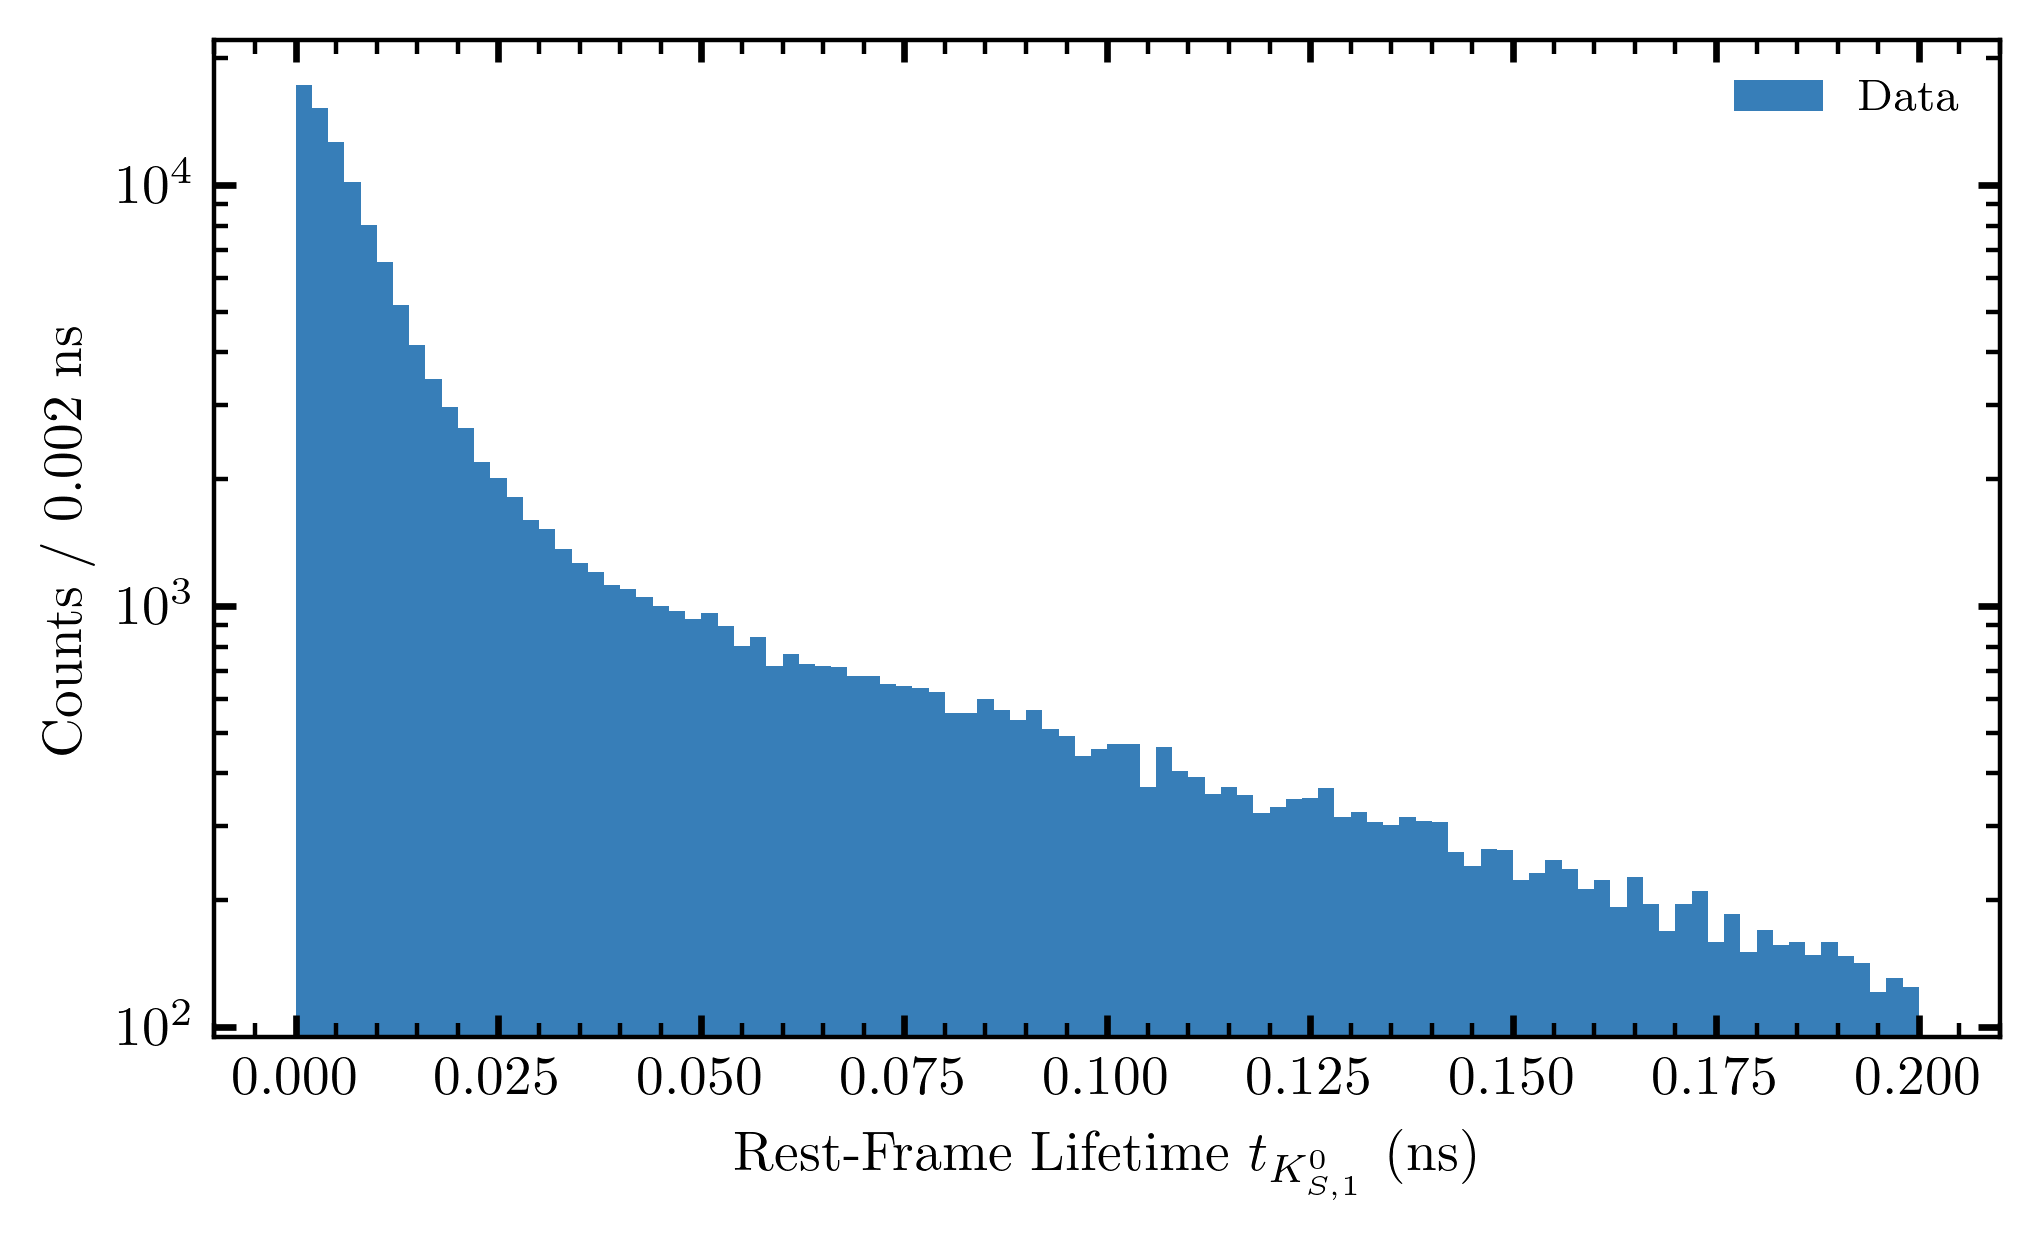
\includegraphics[width=1\linewidth]{rfl_data_chisqdof_3.0.png}
      \caption{}
      \label{fig:rfl-data}
    \end{subfigure}
    \begin{subfigure}[b]{.7\columnwidth}
      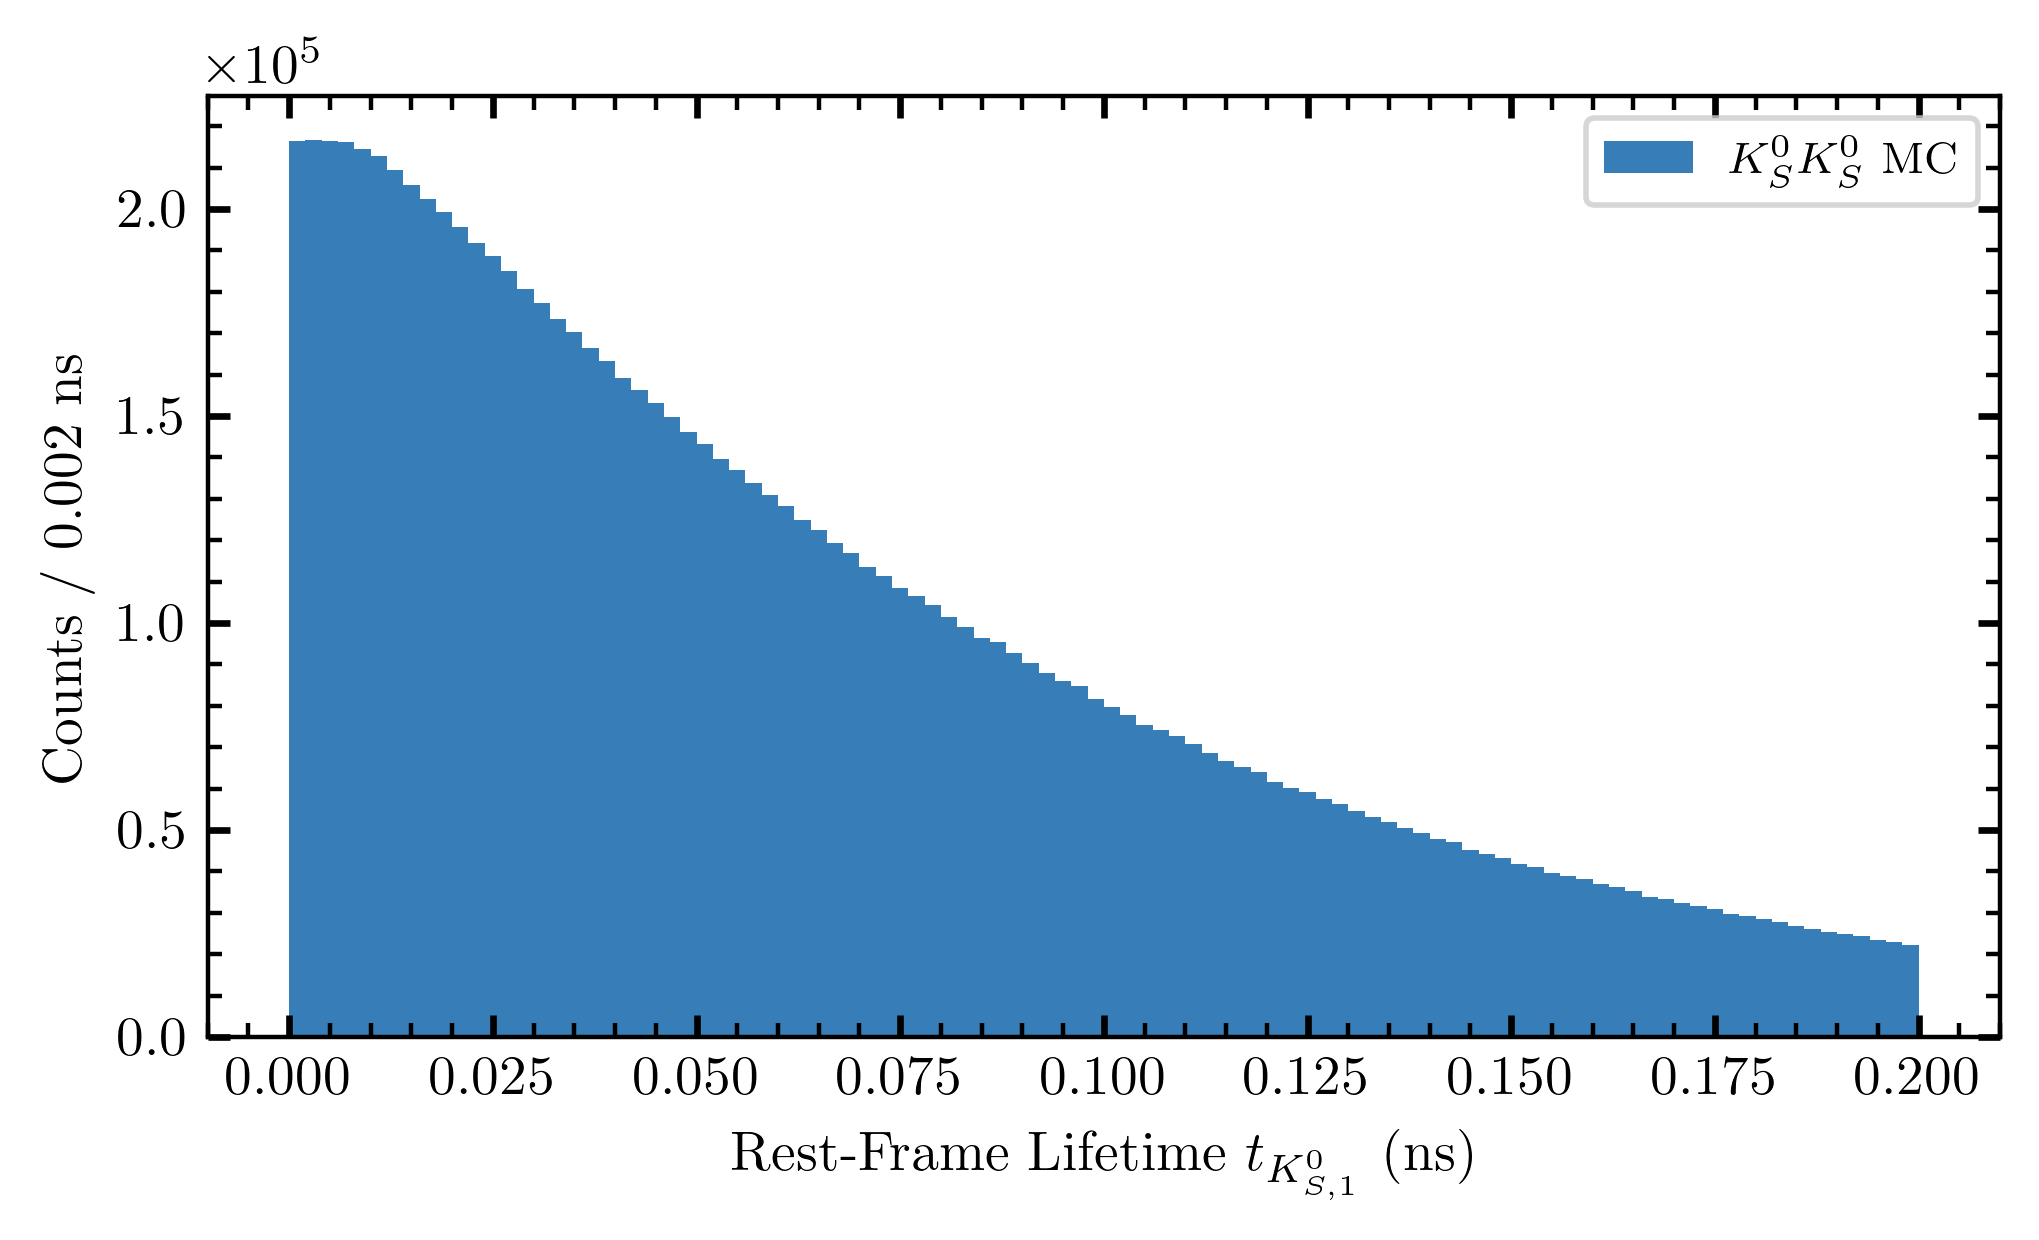
\includegraphics[width=1\linewidth]{rfl_accmc_chisqdof_3.0.png}
      \caption{}
      \label{fig:rfl-accmc}
    \end{subfigure}
    \begin{subfigure}[b]{.7\columnwidth}
      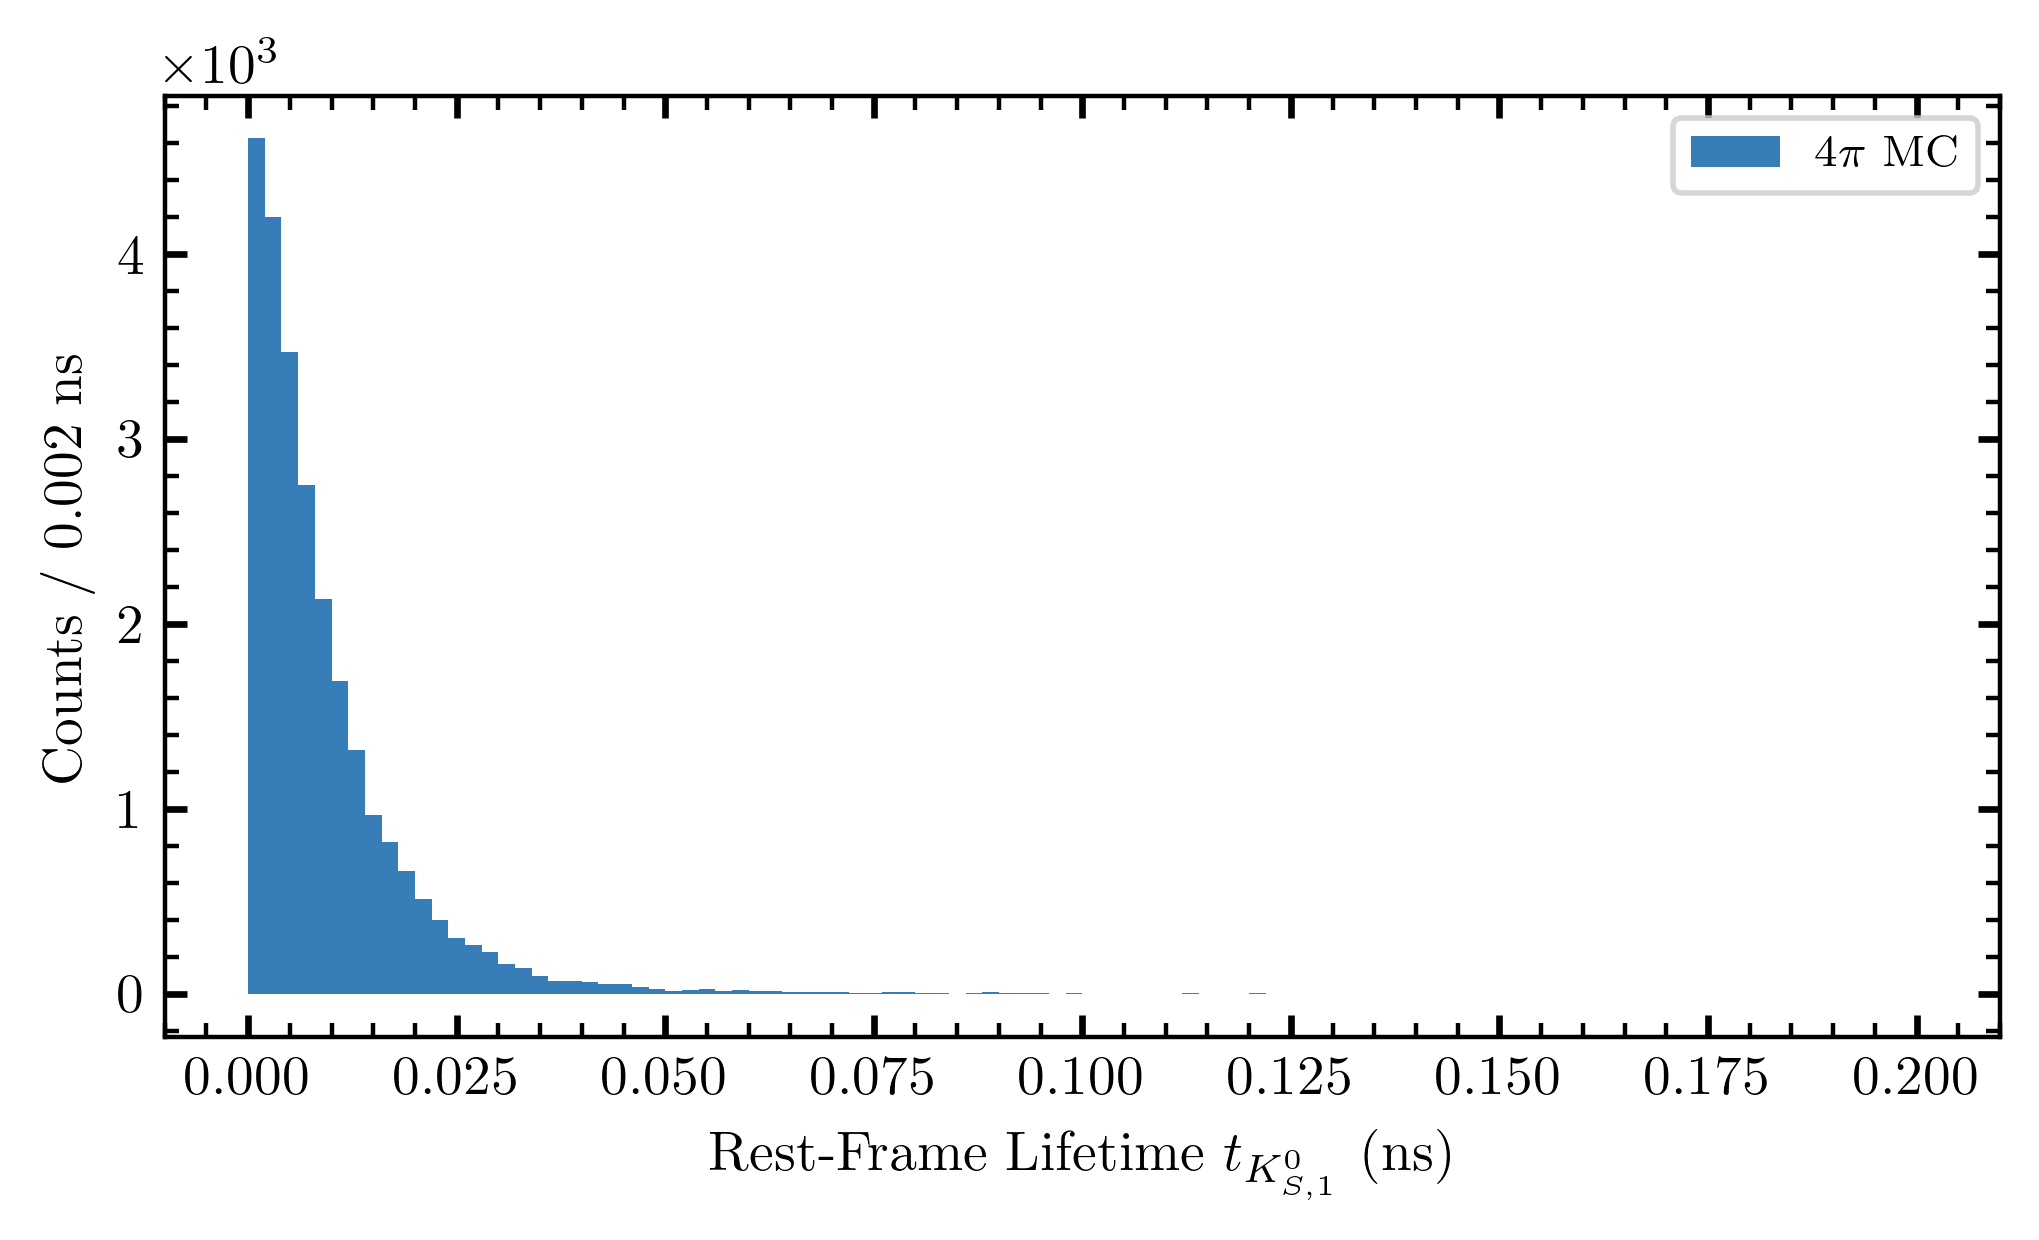
\includegraphics[width=1\linewidth]{rfl_bkgmc_chisqdof_3.0.png}
      \caption{}
      \label{fig:rfl-bkgmc}
    \end{subfigure}
  \end{center}
  \caption{The rest-frame lifetime of kaons in (a) data, (b) signal Monte Carlo, and (c) background Monte Carlo. The data distribution clearly contains two exponential slopes: a peak which resembles the $4\pi$ Monte Carlo distribution, and a tail of true $K_S^0$s which resembles the signal Monte Carlo.}\label{fig:rfl-pre-splot}
\end{figure}

For all of the statistical weighting methods which will be mentioned here, we need some model for the signal and background probability distribution functions (PDFs) for some ``discriminating'' variable. This variable is called ``discriminating'' because it the variable for which we know the shape of these distributions beforehand. The usual example is a ``bump-on-a-background'', in which the discriminating variable may be a mass distribution ($m$) where signal events show up as a peaking structure while background events are more uniformly distributed. In such situations, it is common to use the extremes of the mass distribution (sidebands) as estimates of the background everywhere, weighting these events negatively while the events in the peak are weighted positively (a sideband subtraction). Rather than specifying peak and sideband regions, we can fit the mass distribution to some mixture of a signal (peak) PDF $f_S(m)$ and a background (flat) PDF $f_B(m)$. From such a fit, we obtain estimated number of signal ($N_S$) and background ($N_B$) events in our dataset (and possibly some shape parameters for the signal and background PDFs). We could then assign weights to each event as in \Cref{eq:inplot-weights-mass},

\begin{equation}
  w(m) = \frac{N_S f_S(m)}{N_S f_S(m) + N_B f_B(m)}
  \label{eq:inplot-weights-mass}
\end{equation}

We might want to look at the ``signal'' inPlots for the decay angles $\theta$ and $\varphi$ (control variables) in the helicity system after calculating the inPlot weights from a fit to the mass distribution (discriminating variable). However, as shown by Pivk and Le Diberder\cite{pivk_splot_2005}, we can only use inPlot in cases where the control variables are totally correlated with the discriminating variable\footnote{In practice, more than one discriminating variable can be used.} $y$. In other words, our example would only be valid if $\theta = \theta(m)$ and $\phi = \phi(m)$. For the time being, let us assume that this is not the case, and that we wish to use the distribution of some variable which is totally uncorrelated with the variables we are plotting and analyzing\footnote{Total (un)correlation is a very strict requirement, but we will later see that small modifications to the sPlot method can permit amounts of correlation between the two extremes.}. A correction term can be applied to give us the sPlot version of \Cref{eq:inplot-weights-mass},

\begin{equation}
  w(y) = \tilde{w}(y)\frac{V_{SS}f_S(y) + V_{SB}f_B(y)}{N_S f_S(y) + N_B f_B(y)},\quad \text{where } V^{-1}_{ij} = \sum_{y} \frac{\tilde{w}(y)f_i(y)f_j(y)}{\left(N_S f_S(y) + N_B f_B(y)\right)^2}
  \label{eq:splot-weights}
\end{equation}

where $y$ represents any set of discriminating variables (not necessarily a mass), and $\tilde{w}(y)$ is any pre-existing weight associated with the event (weights from accidental subtraction, for instance). The $V^{-1}$ matrix can also be understood as the covariance matrix between the free parameters $N_S$ and $N_B$ in the fit of the signal-background mixture, $V^{-1}_{ij} = -N\pdv[2]{\ln\mathcal{L}}{N_i}{N_j}$, although there is reason to believe that direct calculation by inverting the Hessian matrix from the fit will lead to less accurate results than the manual calculation method given in \Cref{eq:splot-weights}\cite{dembinski_custom_2022}.

Now that we have a method of assigning weights, we must pick the discriminating variables. As mentioned, these weighting methods work well on the classic ``bump-on-a-background'' distributions because it is easy to identify the signal and background PDFs, but because the mass of the kaons is constrained in the kinematic fit, the fitted mass of each kaon is just a $\delta$-function and combination of measured masses for each $\pi^+\pi^-$ pair will yield a Normal distribution with little to no apparent background (by construction), so we must be a bit more clever in selecting discriminating variables. By examining the BGGEN analysis done in {\color{red}[TODO: PREVIOUS SECTION]}, we can see that most likely sources of background arise when the intermediate kaons are absent from the reaction: $\gamma p \to 4\pi p$. This reaction has the $K_SK_S$ final state, so pairs of pions which reconstruct close enough to kaons will be almost indistinguishable in the data. However, they differ in one key way, namely that the $K_S$ intermediate contains a strange quark while the $\pi^+\pi^-$ decay state does not, so such a decay must occur via the weak interaction, which is notably slower than the strong interaction which would produce pion pairs with no intermediate kaon. In other words, while the signal's rest-frame lifetime distribution should have an exponential slope near the $K_S$ lifetime, the background would theoretically have nearly zero rest-frame lifetime for every event, or a much smaller exponential slope in practice\footnote{An exponential distribution is just what best fits the rest-frame lifetime distribution in the $4\pi$ Monte Carlo and has no physical implication.}.

Therefore, we will begin by generating both a signal and background dataset in Monte Carlo. We then interpret both datasets as if they were our desired channel by running them through the GlueX reconstruction and reaction filter, as well as all of our selections up to this point. We can then fit the rest-frame lifetime of each dataset to an exponential model,

\begin{equation}
  f(t; \lambda) = \lambda \exp{-\lambda t}
  \label{eq:splot-exponential}
\end{equation}
where $\lambda \equiv 1/\tau$, the lifetime of the kaon in question. Since we have two independently decaying kaons, we should really form a joint distribution for both, where we will assume each kaon has the same average lifetime:
\begin{equation}
  f(t_1, t_2; \lambda) = \lambda^2 \exp{-\lambda t_1}\exp{-\lambda t_2}
  \label{eq:splot-exponential_joint}
\end{equation}
Both the signal and background distributions can be modeled in this way, giving us only two free parameters, $\lambda_S$ and $\lambda_B$ for the signal and background respectively, to fit.

We can then use a mixture of exponential distributions with both signal and background slopes to fit the entire dataset:
\begin{equation}
  f(t_1, t_2; z, \lambda_S, \lambda_B) \equiv z f(t_1, t_2; \lambda_S) + (1-z) f(t_1, t_2; \lambda_B)
  \label{eq:splot-mixture}
\end{equation}

where $z$ is the signal fraction of the total number of events $N$. From its fit value, we can determine values of $N_S = z\cdot N$ and $N_B = (1-z)\cdot N$ to use in \Cref{eq:splot-weights} and complete the weighting procedure. We can perform this fit by minimizing the negative log-likelihood function,

\begin{equation}
  -2\ln\mathcal{L}(z, \lambda_S, \lambda_B) = -2\sum_i^N \tilde{w}_i \ln f(t_{1,i}, t_{2,i}; z, \lambda_S, \lambda_B)
  \label{eq:splot-nll}
\end{equation}

where again, we include any pre-existing weights $\tilde{w}$ in the fit.

\subsection{Non-Factorizing sPlot}\label{sec:non-factorizing-splot}

Over the course of the previous discussion, it was assumed that the discriminating variables, $t_1$ and $t_2$, were statistically independent from the control variables we wish to use in later analyses. The set of control variables must include all variables we use as inputs to the partial-wave analysis in \Cref{ch:partial-wave-analysis}, including the invariant mass $m$ of the $K_S^0K_S^0$ system and the helicity angles $\theta$ and $\varphi$ of the decay. We should now confirm that the rest-frame lifetimes are totally uncorrelated with these control variables (in other words, show that they are statistically independent). To test for statistical independence between $t_{1,2}$ and a given control variable, we first split our dataset into $M$ evenly-spaced quantiles in that control variable, which ensures each bin gets roughly the same number of events. Next, we calculate the likelihood of a null hypothesis which assumes the variables are statistically independent by fitting all datasets simultaneously with shared $\lambda_S$ and $\lambda_B$ parameters. We then calculate the likelihood of an alternative hypothesis, which assumes statistical dependence, by finding the joint likelihood of independent fits of $\lambda_S$ and $\lambda_B$ over each quantile. The result of these fits can be formulated as a likelihood ratio,

\begin{equation}
  \Lambda = -2\ln\frac{\sup \mathcal{L}_{H_0}}{\sup \mathcal{L}_{H_1}} = -2\ln\frac{\sup \prod_i^M \mathcal{L}_i(z_i, \lambda_S, \lambda_B)}{\sup \prod_i^M \mathcal{L}_i(z_i, \lambda_{S,i}, \lambda_{B,i})}
  \label{eq:independence-test}
\end{equation}

where $\mathcal{L}_{H_0}$ and $\mathcal{L}_{H_1}$ are the likelihoods of the null and alternative hypotheses respectively, the supremum indicates we are maximizing these likelihoods (in a maximum likelihood fit), the product $\prod_i^M$ iterates over each quantile of data in the given control variable, and $\mathcal{L}_i$ is the likelihood evaluated over data in the $i$th quantile. $\Lambda$ is $\chi^2$ distributed with $2M - 2$ degrees of freedom (the difference between $M + 2$ free parameters in the null hypothesis, a signal fraction $z_i$ for each quantile plus the two exponential slopes shared across all quantiles, and $3M$ in the alternative hypothesis, a signal fraction and two exponential slopes for each quantile). The factor of $2$ is required because $\ln\mathcal{L}(\theta_1,...,\theta_i) \sim -\frac{1}{2}\chi^2_i$ asymptotically with sample size, according to Wilks' theorem. We can obtain a $p$-value representing the likelihood of the null hypothesis being true by evaluating the $p$-value:

\begin{equation}
  p = 1 - F_{\chi^2_{2M-2}}(\Lambda)
  \label{eq:significance-test}
\end{equation}

where $F_{\chi^2_{2M-2}}(\Lambda)$ is the cumulative distribution function of a $\chi^2$ distribution with $2M-2$ degrees of freedom. Following this procedure for the invariant mass of $K_S^0K_S^0$\footnote{No significant statistical dependence was found for the helicity angles.}, the $p$-values for each number of quantiles can be seen in the first row of \Cref{tab:factorization-results} and in \Cref{fig:data-factorization-fit}, which depicts the case with four quantiles. The calculated $p$-values tend to be very small, implying that we should reject the null hypothesis and accept that the discriminating (rest-frame lifetime) and control (invariant mass of $K_S^0K_S^0$) variables are not statistically independent. This means we cannot use a traditional sPlot to weight our data.

Fortunately, the process for obtaining the correct weights is straightforward, we simply allow for more than one signal and background component in the fit and sum over all signal components when we calculate the final weight values~\cite{dembinski_custom_2022}. Since the weights corresponding to each signal component in the sPlot can be added to each other to obtain a joint weight~\cite{pivk_splot_2005}, \Cref{eq:splot-weights} can be extended to allow multiple signal and background components:

\begin{equation}
  w(x) = \frac{\sum_{j} V_{S_0 j}f_j(x)}{\sum_{k}N_kf_k(x)} + ... + \frac{\sum_{j} V_{S_n j}f_j(x)}{\sum_{k}N_kf_k(x)},\quad \text{where } V_{ij}^{-1} = \sum_{x} \frac{f_i(x)f_j(x)}{\left(\sum_{k} N_kf_k(x)\right)^2}
  \label{eq:splot-weights-factorizing}
\end{equation}

and $S_i$ are the indices of the signal components.

We can further verify the need for non-factorizing sPlot by performing the factorization test described in \Cref{eq:independence-test,eq:significance-test} to the signal and background Monte Carlo, with a slight modification to the number of free parameters, since we only need to fit either a signal or background component rather than a mixture:

\begin{equation}
  p = 1 - F_{\chi^2_{M-1}} \quad\text{where }\Lambda = -2\ln\frac{\sup\prod_i^M \mathcal{L}_i(\lambda)}{\sup\prod_i^M \mathcal{L}_i(\lambda_i)}
  \label{eq:independence-test-mc}
\end{equation}

The results of these tests over the signal and background Monte Carlo can also be found in the last two rows of \Cref{tab:factorization-results} and are visualized for four quantiles in \Cref{fig:mc-factorization-fits}. Again, the significantly small $p$-values justify the use of non-factorizing sPlot across both the signal and background components, meaning that we need at least two signal and two background components in the final sPlot weighting.

\begin{table}
  \begin{center}
    \begin{tabular}{cccc}\toprule
       & \multicolumn{3}{c}{\# quantiles} \\\cmidrule(lr){2-4}
       & 2 & 3 & 4 \\
       Data Type & $p$ & $p$ & $p$ \\\midrule
      Data  & $1.26 \times 10^{-101}$ & $9.94 \times 10^{-103}$ & $4.49 \times 10^{-112}$\\
      $K_S^0K_S^0$ MC  & $<2.23\times 10^{-308}$ & $<2.23\times 10^{-308}$ & $<2.23\times 10^{-308}$\\
      $4\pi$ MC  & $1.87 \times 10^{-05}$ & $1.00 \times 10^{-04}$ & $7.38 \times 10^{-05}$\\\bottomrule
    \end{tabular}
    \caption{The probability of accepting the null hypothesis (that the rest-frame lifetime is statistically independent of the invariant mass of $K_S^0K_S^0$) for the tests described in \Cref{eq:independence-test} for data and \Cref{eq:independence-test-mc} for Monte Carlo with the given number of quantiles. All values are calculated with a $\chi^2_\nu < 3.0$ selection on each type of data over all run period combined. Values listed as $<2.23 \times 10^{-308}$ are nonzero but smaller than the smallest representable 64-bit floating point number}\label{tab:factorization-results}
  \end{center}
\end{table}

\begin{figure}
  \begin{center}
    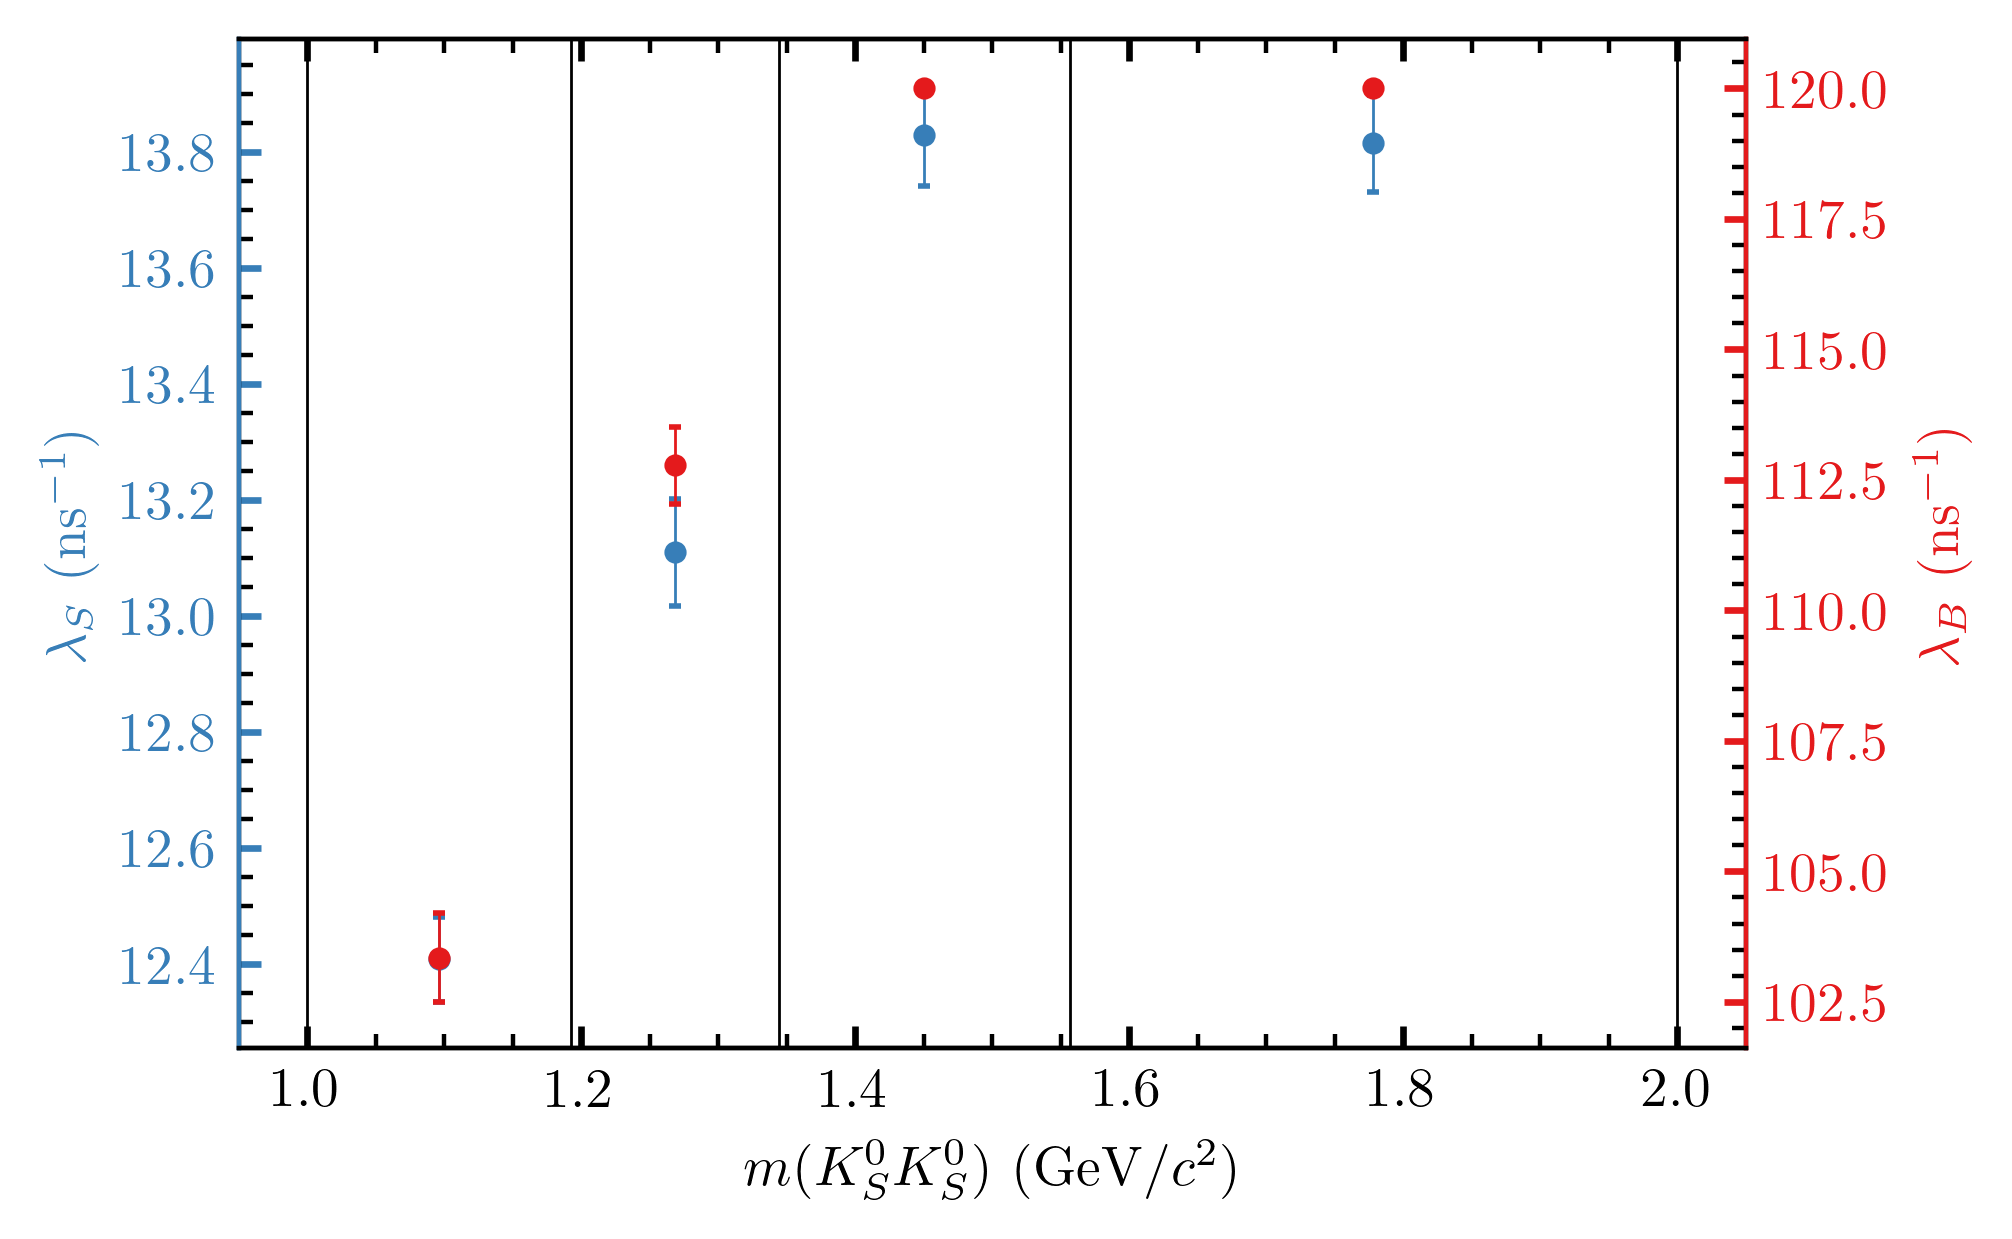
\includegraphics[width=.8\columnwidth]{factorization_plot_data_chisqdof_3.0_4_quantiles.png}
  \end{center}
  \caption{Exponential slopes from fits over four quantiles in $m(K_S^0K_S^0)$ ($x$-axis) to a mixture of signal (left $y$-axis) and background (right $y$-axis) components. These fits show a definite statistical dependence between rest-frame lifetime and the invariant mass of $K_S^0K_S^0$, as described in \Cref{tab:factorization-results}. All values are calculated with a KinFit $\chi^2_\nu < 3.0$ selection on each type of data over each run period.}\label{fig:data-factorization-fit}
\end{figure}

\begin{figure}
  \begin{center}
    \begin{subfigure}[b]{.8\columnwidth}
      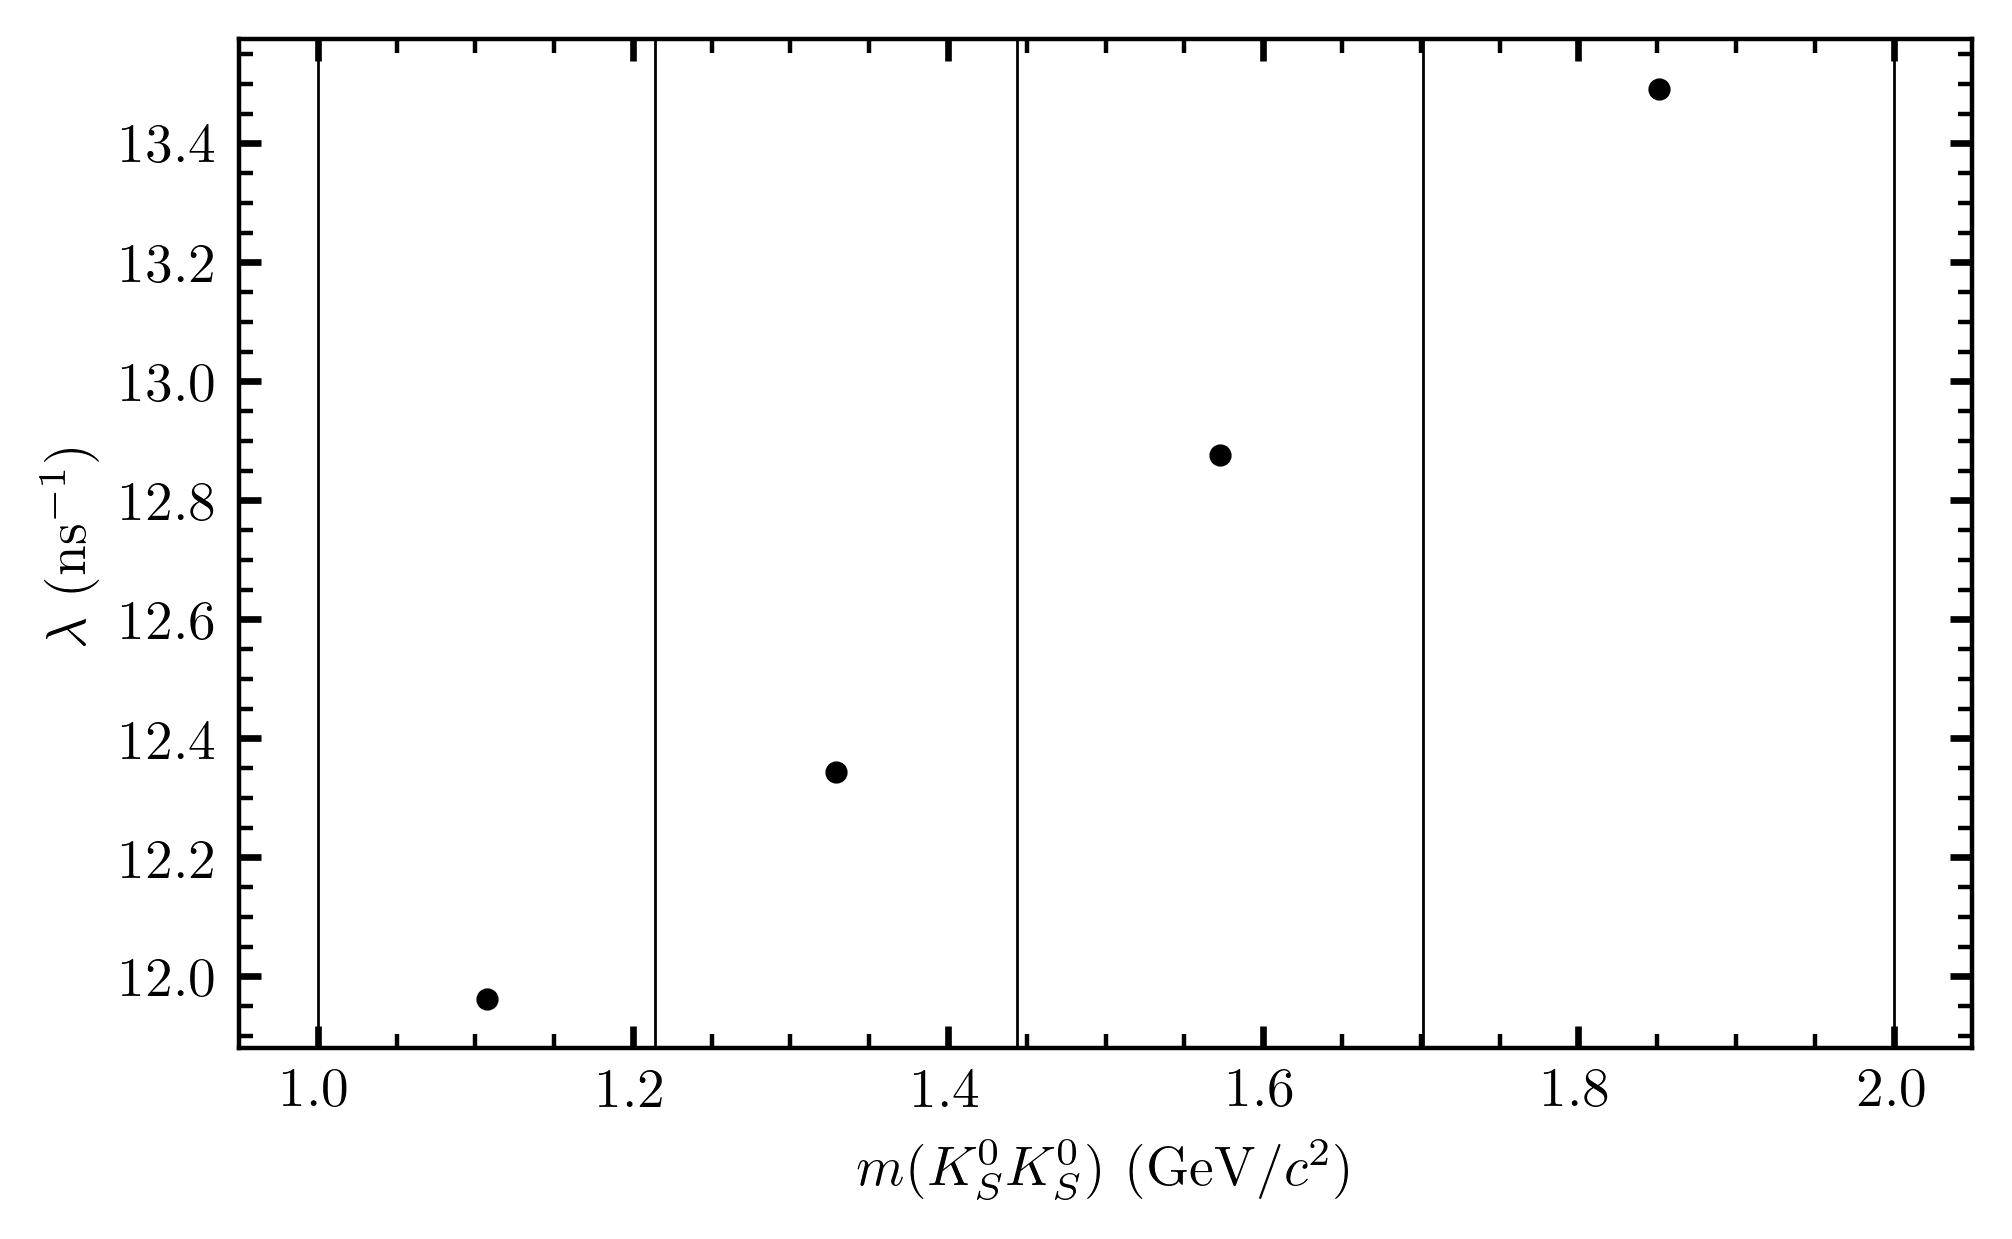
\includegraphics[width=1\linewidth]{factorization_plot_accmc_chisqdof_3.0_4_quantiles.png}
      \caption{}
      \label{fig:mc-factorization-fits-a}
    \end{subfigure}
    \begin{subfigure}[b]{.8\columnwidth}
      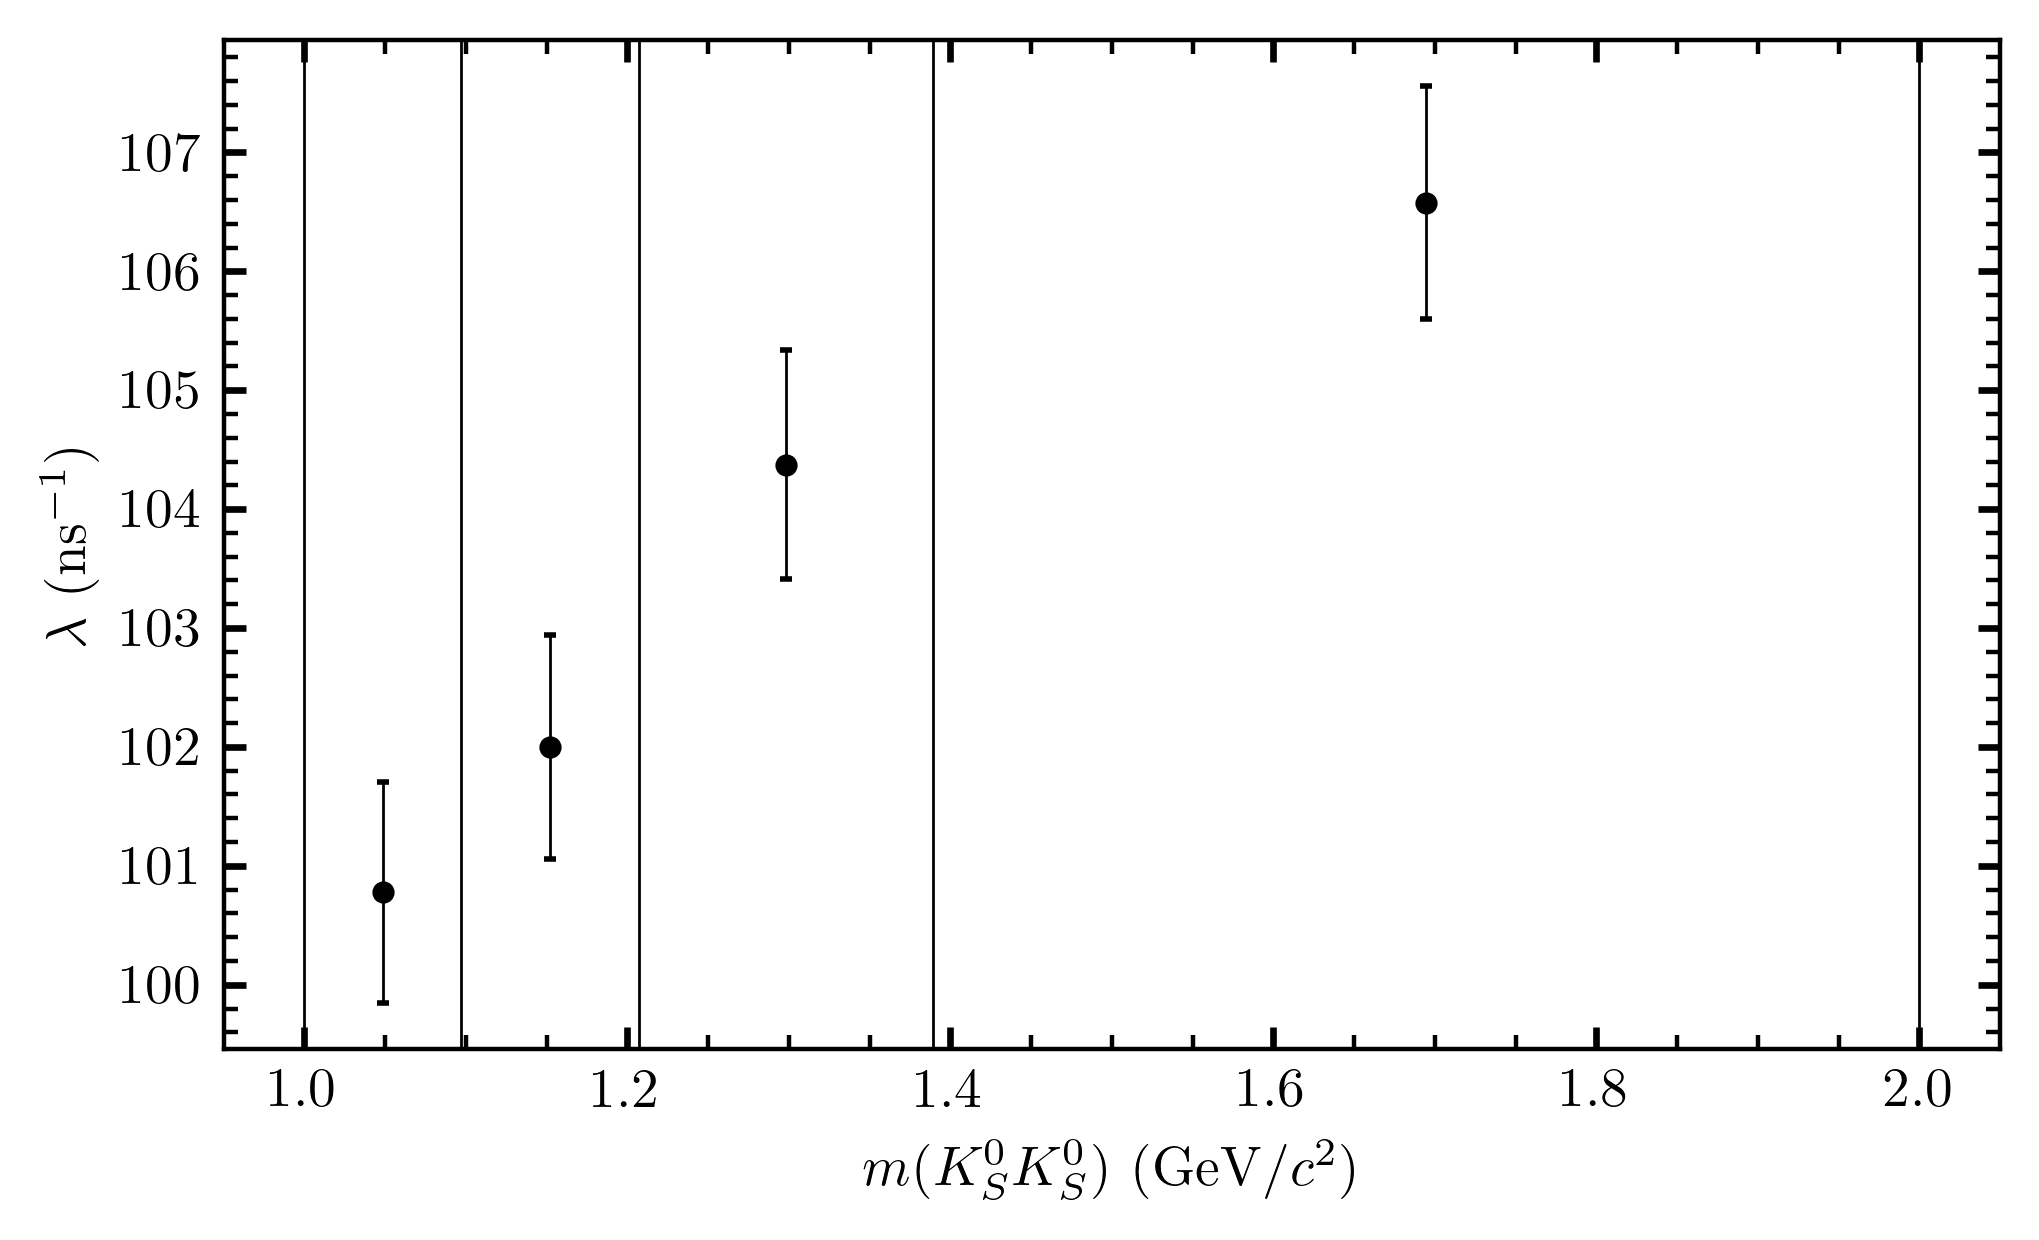
\includegraphics[width=1\linewidth]{factorization_plot_bkgmc_chisqdof_3.0_4_quantiles.png}
      \caption{}
      \label{fig:mc-factorization-fits-b}
    \end{subfigure}
  \end{center}
  \caption{Exponential slopes from fits over four quantiles in $m(K_S^0K_S^0)$ ($x$-axis) of the (a) signal and (b) background Monte Carlo rest-frame lifetime distributions. Both show a definite statistical dependence between rest-frame lifetime and the invariant mass of $K_S^0K_S^0$, as described in \Cref{tab:factorization-results}. All values are calculated with a KinFit $\chi^2_\nu < 3.0$ selection on each type of data over each run period.}\label{fig:mc-factorization-fits}
\end{figure}

\subsection{Application of Weights}\label{sec:application-of-weights}

The only thing left to do is determine how many signal and background components we should use in the weighting procedure. To this end, we now turn to the Monte Carlo simulations of the signal and $4\pi$-background. By choosing a number of quantiles in invariant mass corresponding to the number of components, we can fit single exponential distributions to each quantile in the simulated signal and background. For instance, if we chose to use two signal components and three background components, we would divide the signal Monte Carlo into two quantiles and the background Monte Carlo into three, and fit each quantile to an exponential distribution to obtain a set of two $\lambda_S$ and three $\lambda_B$ values. The resulting $\lambda_S$ and $\lambda_B$ values could then be used as a starting point for a multi-component fit to the data. Alternatively, both the signal and background or just the signal could be fixed to the values from the fits to simulations, and only the yields (or the yields and background $\lambda$s) would be allowed to float in the fit to data. We will refer to the first case, where the fit parameters from Monte Carlo are free, as $A$, the case where the signal $\lambda$s are fixed as $B$, and the case where all $\lambda$s are fixed (and the only floating parameters are the yields of each component) as $C$. To select a model, we can use the relative Akaike Information Criterion (AIC)~\cite{akaike_information_1998} and Bayesian Information Criterion (BIC)~\cite{schwarz_estimating_1978}:
\begin{alignat}{2}
  r\text{AIC} &\equiv \text{AIC} - \text{AIC}_\text{min} \quad\text{where } \text{AIC} &&\equiv 2k - 2\ln\mathcal{L} \\
  r\text{BIC} &\equiv \text{BIC} - \text{BIC}_\text{min} \quad\text{where } \text{BIC} &&\equiv k\ln{N} - 2\ln\mathcal{L} \\
  \label{eq:information-criteria}
\end{alignat}
where $k$ is the number of free parameters and $N$ is the number of events in the dataset. The optimal model will minimize these criteria. In \Cref{tab:splot-model-results}, all of the relative AIC and BIC values are shown. Excluding cases with only one signal or background component (restricting to models which have non-factorizing signal and background components), the minimizing values for most run periods tend to use two or three signal and two background components, and they both use method $B$, where the signal components are fixed to values obtained from Monte Carlo while the background components are initialized at Monte Carlo values but allowed to float in the fit. We will use the minimal non-factorizing model, method $B$ with two signal and two background components, denoted $B(2,2)$, as our weighting method. See \Cref{fig:splot-data-fit} for the result of this fit. The selection of method $B$ is also interesting as it could describe a case where another background which is not modeled in the background Monte Carlo is present and has a similar exponential slope. Since these slopes are free in the fit to the data, they may anticipate this unknown slope better than the fixed case (method $C$), and method $B$ also explicitly assumes the Monte Carlo for true signal kaons is correct and fixes their component slopes (unlike method $A$).

\begin{table}
  \begin{center}
    \begin{tabular}{ccccc}\toprule
    & \multicolumn{2}{c}{\# Components} & \\\cmidrule(lr){2-3}
      Method & Signal & Background & $r\text{AIC}$ & $r\text{BIC}$\\\midrule
      $A$ & $1$ & $1$ & \underline{$0.000$} & \underline{$0.000$}\\
       & $1$ & $2$ & $4.000$ & $25.420$\\
       & $1$ & $3$ & $8.004$ & $50.843$\\
       & $2$ & $1$ & $4.000$ & $25.420$\\
       & $2$ & $2$ & $8.000$ & $50.839$\\
       & $2$ & $3$ & $12.003$ & $76.261$\\
       & $3$ & $1$ & $8.000$ & $50.839$\\
       & $3$ & $2$ & $12.002$ & $76.261$\\
       & $3$ & $3$ & $16.002$ & $101.681$\\\midrule
      $B$ & $1$ & $1$ & $312.365$ & $301.655$\\
       & $1$ & $2$ & $213.928$ & $224.638$\\
       & $1$ & $3$ & $217.324$ & $249.453$\\
       & $2$ & $1$ & $23.929$ & $23.929$\\
       & $2$ & $2$ & $9.758$ & \fcolorbox{red}{white}{$31.177$}\\
       & $2$ & $3$ & $13.629$ & $56.468$\\
       & $3$ & $1$ & $2.001$ & $12.711$\\
       & $3$ & $2$ & \fcolorbox{red}{white}{$6.004$} & $38.134$\\
       & $3$ & $3$ & $10.002$ & $63.551$\\\midrule
      $C$ & $1$ & $1$ & $1695.033$ & $1673.614$\\
       & $1$ & $2$ & $1305.143$ & $1294.433$\\
       & $1$ & $3$ & $1197.528$ & $1197.528$\\
       & $2$ & $1$ & $1661.600$ & $1650.890$\\
       & $2$ & $2$ & $1245.238$ & $1245.238$\\
       & $2$ & $3$ & $1128.344$ & $1139.053$\\
       & $3$ & $1$ & $1661.070$ & $1661.070$\\
       & $3$ & $2$ & $1247.365$ & $1258.074$\\
       & $3$ & $3$ & $1131.169$ & $1152.588$\\\bottomrule
    \end{tabular}
    \caption{Relative AIC and BIC values for each fitting method. The absolute minimum values in each column are underlined, and the minimums excluding models with only one signal or background component are boxed.}\label{tab:splot-model-results}
  \end{center}
\end{table}

\begin{figure}
  \begin{center}
    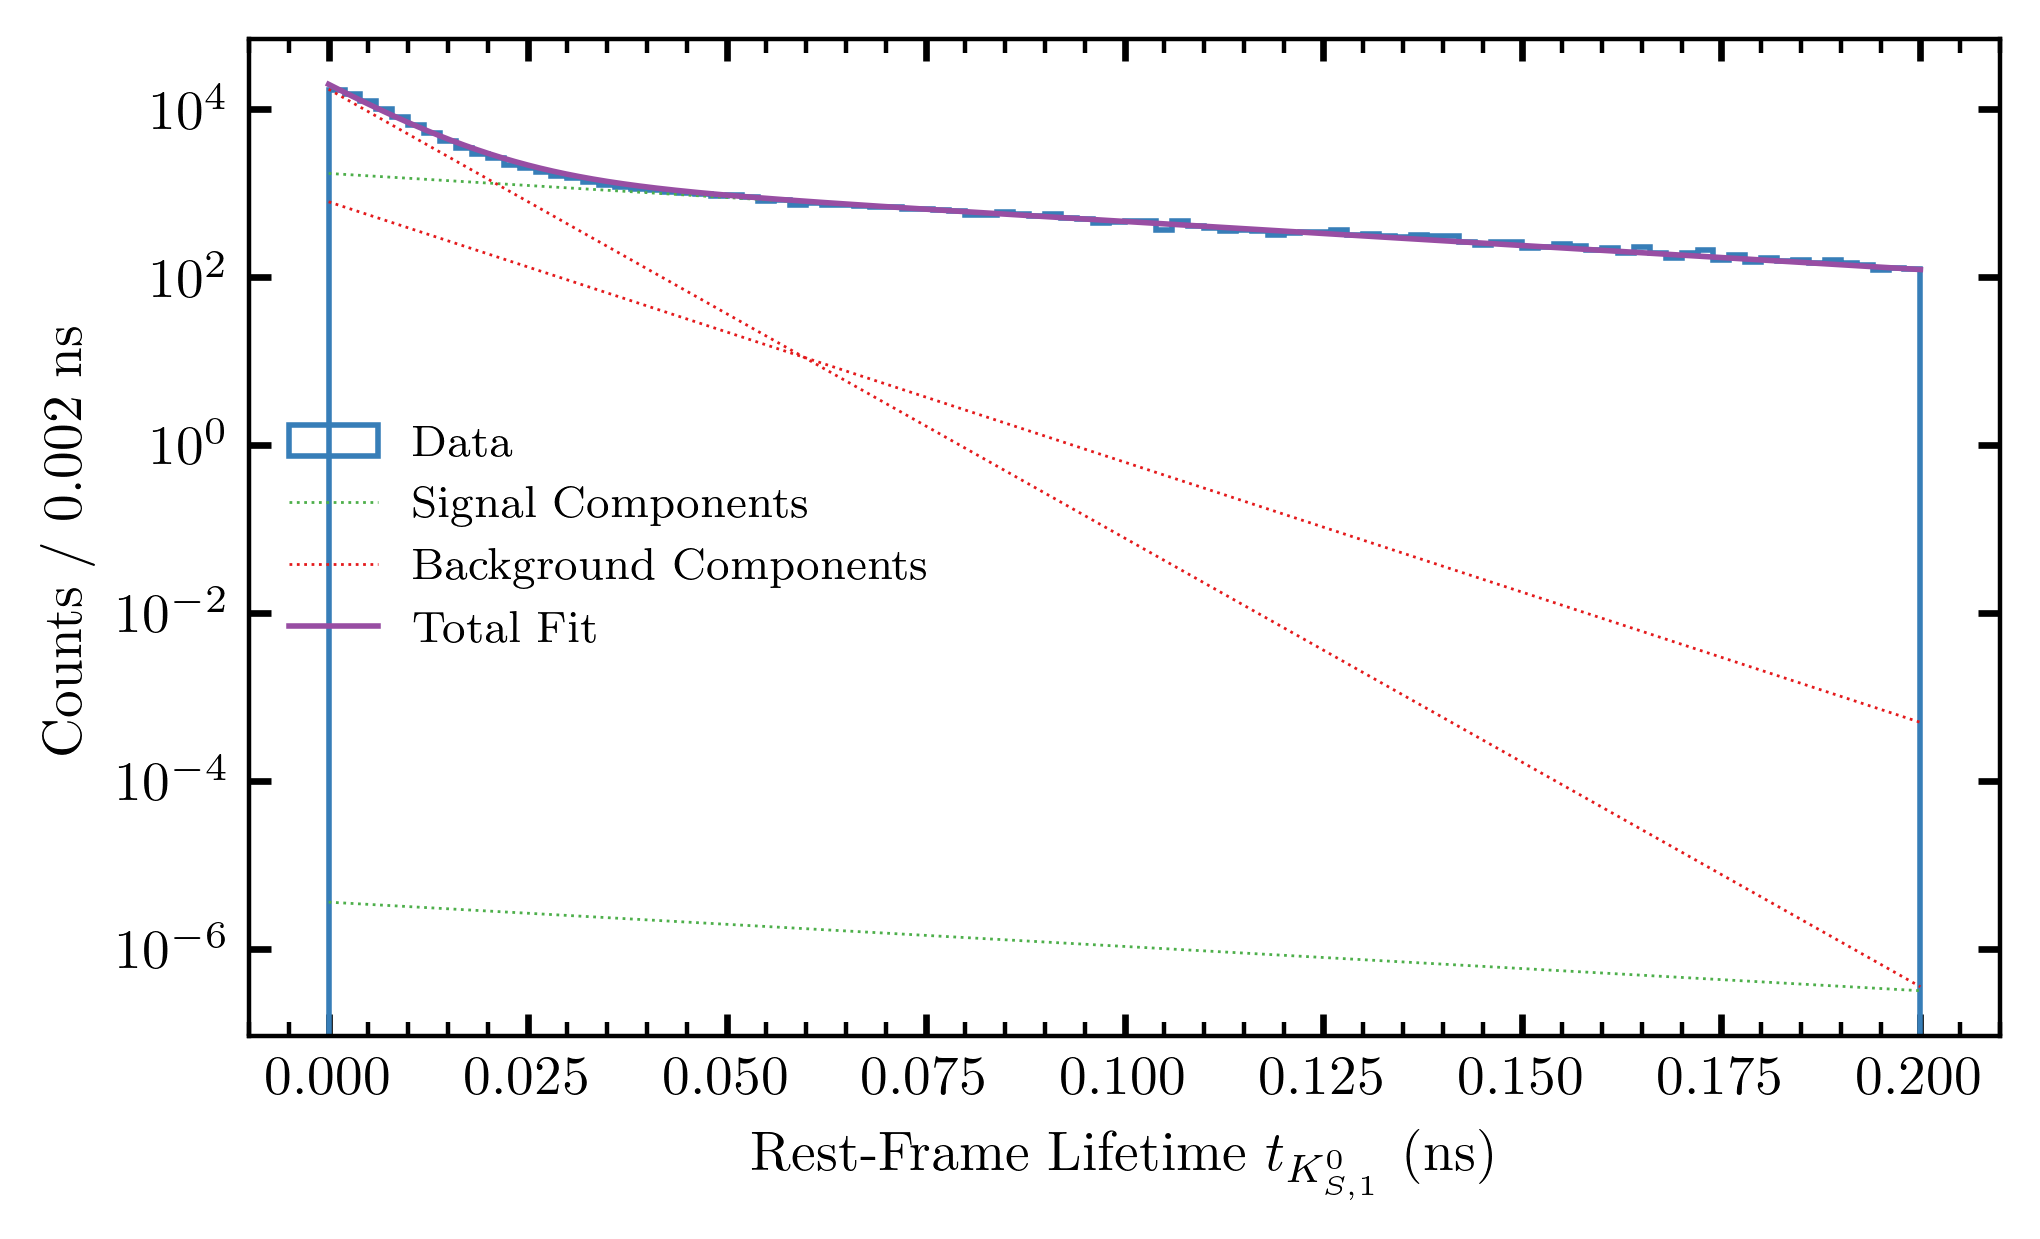
\includegraphics[width=.8\columnwidth]{splot_fit_data_chisqdof_3.0_splot_B_2s_2b.png}
  \end{center}
  \caption{Fit of \Cref{eq:splot-mixture} to data using method $B(2,2)$. True kaon events are prominent in the tail of the distribution, whereas background events peak strongly near zero. All values are calculated with a KinFit $\chi^2_\nu < 3.0$ selection on each type of data over each run period. The second signal component tends to be very small but non-zero across all datasets.}\label{fig:splot-data-fit}
\end{figure}

